%% abtex2-modelo-artigo.tex, v-1.9.7 laurocesar
%% Copyright 2012-2018 by abnTeX2 group at http://www.abntex.net.br/ 
%%
%% This work may be distributed and/or modified under the
%% conditions of the LaTeX Project Public License, either version 1.3
%% of this license or (at your option) any later version.
%% The latest version of this license is in
%%   http://www.latex-project.org/lppl.txt
%% and version 1.3 or later is part of all distributions of LaTeX
%% version 2005/12/01 or later.
%%
%% This work has the LPPL maintenance status `maintained'.
%% 
%% The Current Maintainer of this work is the abnTeX2 team, led
%% by Lauro César Araujo. Further information are available on 
%% http://www.abntex.net.br/
%%
%% This work consists of the files abntex2-modelo-artigo.tex and
%% abntex2-modelo-references.bib
%%

% ------------------------------------------------------------------------
% ------------------------------------------------------------------------
% abnTeX2: Modelo de Artigo Acadêmico em conformidade com
% ABNT NBR 6022:2018: Informação e documentação - Artigo em publicação 
% periódica científica - Apresentação
% ------------------------------------------------------------------------
% ------------------------------------------------------------------------
\PassOptionsToPackage{hyphens}{url}
\documentclass[
	% -- opções da classe memoir --
	article,			% indica que é um artigo acadêmico
	11pt,				% tamanho da fonte
	oneside,			% para impressão apenas no recto. Oposto a twoside
	a4paper,			% tamanho do papel. 
	% -- opções da classe abntex2 --
	%chapter=TITLE,		% títulos de capítulos convertidos em letras maiúsculas
	%section=TITLE,		% títulos de seções convertidos em letras maiúsculas
	%subsection=TITLE,	% títulos de subseções convertidos em letras maiúsculas
	%subsubsection=TITLE % títulos de subsubseções convertidos em letras maiúsculas
	% -- opções do pacote babel --
	english,			% idioma adicional para hifenização
	brazil,				% o último idioma é o principal do documento
	sumario=tradicional	
	]{abntex2}


% ---
% PACOTES
% ---

% ---
% Pacotes fundamentais 
% ---
\usepackage{lmodern}			% Usa a fonte Latin Modern
\usepackage[T1]{fontenc}		% Selecao de codigos de fonte.
\usepackage[utf8]{inputenc}		% Codificacao do documento (conversão automática dos acentos)
\usepackage{indentfirst}		% Indenta o primeiro parágrafo de cada seção.
\usepackage{nomencl} 			% Lista de simbolos
\usepackage{color}				% Controle das cores
\usepackage{graphicx}			% Inclusão de gráficos
\usepackage{microtype} 			% para melhorias de justificação
% ---
		
% ---
% Pacotes adicionais, usados apenas no âmbito do Modelo Canônico do abnteX2
% ---
\usepackage{lipsum}				% para geração de dummy text
% ---
		
% ---
% Pacotes de citações
% ---
\usepackage[brazilian,hyperpageref]{backref}	 % Paginas com as citações na bibl
\usepackage[alf]{abntex2cite}	% Citações padrão ABNT
% ---

% ---
% Configurações do pacote backref
% Usado sem a opção hyperpageref de backref
\renewcommand{\backrefpagesname}{Citado na(s) página(s):~}
% Texto padrão antes do número das páginas
\renewcommand{\backref}{}
% Define os textos da citação
\renewcommand*{\backrefalt}[4]{
	\ifcase #1 %
		Nenhuma citação no texto.%
	\or
		Citado na página #2.%
	\else
		Citado #1 vezes nas páginas #2.%
	\fi}%
% ---

% --- Informações de dados para CAPA e FOLHA DE ROSTO ---
\titulo{Robô de Busca e Salvamento em Desabamentos}
\tituloestrangeiro{Rescue and Save Robot for Collapsed Buildings Enviroment}

\autor{Tiago Soares de Souza Lima\thanks{lima.tss@gmail.com} }

\local{Brasil}
\data{2023}
% ---

% ---
% Configurações de aparência do PDF final

% alterando o aspecto da cor azul
\definecolor{blue}{RGB}{41,5,195}

% informações do PDF
\makeatletter
\hypersetup{
     	%pagebackref=true,
		pdftitle={\@title}, 
		pdfauthor={\@author},
    	pdfsubject={Modelo de artigo científico com abnTeX2},
	    pdfcreator={LaTeX with abnTeX2},
		pdfkeywords={abnt}{latex}{abntex}{abntex2}{atigo científico}, 
		colorlinks=true,       		% false: boxed links; true: colored links
    	linkcolor=blue,          	% color of internal links
    	citecolor=blue,        		% color of links to bibliography
    	filecolor=magenta,      		% color of file links
		urlcolor=blue,
		bookmarksdepth=4
}
\makeatother
% --- 

% ---
% compila o indice
% ---
\makeindex
% ---

% ---
% Altera as margens padrões
% ---
\setlrmarginsandblock{3cm}{3cm}{*}
\setulmarginsandblock{3cm}{3cm}{*}
\checkandfixthelayout
% ---

% --- 
% Espaçamentos entre linhas e parágrafos 
% --- 

% O tamanho do parágrafo é dado por:
\setlength{\parindent}{1.3cm}

% Controle do espaçamento entre um parágrafo e outro:
\setlength{\parskip}{0.2cm}  % tente também \onelineskip

% Espaçamento simples
\SingleSpacing


% ----
% Início do documento
% ----

\begin{document}


% Seleciona o idioma do documento (conforme pacotes do babel)
%\selectlanguage{english}
\selectlanguage{brazil}

% Retira espaço extra obsoleto entre as frases.
\frenchspacing 

% ----------------------------------------------------------
% ELEMENTOS PRÉ-TEXTUAIS
% ----------------------------------------------------------

%---
%
% Se desejar escrever o artigo em duas colunas, descomente a linha abaixo
% e a linha com o texto ``FIM DE ARTIGO EM DUAS COLUNAS''.
% \twocolumn[    		% INICIO DE ARTIGO EM DUAS COLUNAS
%
%---

% página de titulo principal (obrigatório)
\maketitle


% titulo em outro idioma (opcional)



% resumo em português
\begin{resumoumacoluna}
 Conforme a ABNT NBR 6022:2018, o resumo no idioma do documento é elemento obrigatório. 
 Constituído de uma sequência de frases concisas e objetivas e não de uma 
 simples enumeração de tópicos, não ultrapassando 250 palavras, seguido, logo 
 abaixo, das palavras representativas do conteúdo do trabalho, isto é, 
 palavras-chave e/ou descritores, conforme a NBR 6028. (\ldots) As 
 palavras-chave devem figurar logo abaixo do resumo, antecedidas da expressão 
 Palavras-chave:, separadas entre si por ponto e finalizadas também por ponto.
 
 \vspace{\onelineskip}
 
 \noindent
 \textbf{Palavras-chave}: latex. abntex. editoração de texto.
\end{resumoumacoluna}


% resumo em inglês
\renewcommand{\resumoname}{Abstract}
\begin{resumoumacoluna}
 \begin{otherlanguage*}{english}
   According to ABNT NBR 6022:2018, an abstract in foreign language is optional.

   \vspace{\onelineskip}
 
   \noindent
   \textbf{Keywords}: latex. abntex.
 \end{otherlanguage*}  
\end{resumoumacoluna}

% ]  				% FIM DE ARTIGO EM DUAS COLUNAS
% ---

\begin{center}\smaller
\textbf{Data de submissão e aprovação}: elemento obrigatório. Indicar dia, mês e ano

\textbf{Identificação e disponibilidade}: elemento opcional. Pode ser indicado 
o endereço eletrônico, DOI, suportes e outras informações relativas ao acesso.
\end{center}

% ----------------------------------------------------------
% ELEMENTOS TEXTUAIS
% ----------------------------------------------------------
\textual


% ----------------------------------------------------------
% Introdução
% ----------------------------------------------------------
\section{Introdução}
Robôs de busca e salvamento vem sendo usados desde a resposta ao atentado contra o World Trade Center \cite{Robin2004}. Os robôs são uma ferramenta valiosa para os times de busca e salvamento pois, podem adentrar espaços confinados pequenos demais para humanos, ou que sejam tóxicos, a fim de localizar espaços vazios que possam conter sobreviventes \cite{Robin2004}.

Ainda que no Brasil terremotos capazes de causar danos estruturais as construções e atentados da magnitude do World Trade Center não ocorram, equipes de busca e salvamento (SAR) são empregadas em casos de: desabamento por chuvas \cite{serrana2022}, rompimento de barragens \cite{bruma2019}, desabamento de construções irregulares \cite{rio2021}, ou que possuam problemas de manutenção \cite{sp2020}.

Em \cite{Robin2004} é feita uma análise da utilização dos robôs na resposta ao atentado contra o World Trade Center. Como se tratam de robôs operados remotamente sem nenhuma cognição, sobretudo adaptados de usos militares, nota-se a grande carga de trabalho que é depositada entre o condutor do robô, responsável pela movimentação do robô, e o Analista da Situação, responsável por interpretar os dados vindos dos sensores do robô. Ainda que importantes na operação de busca e salvamento como pode ser visto em  \cite{akgun2022using} a falta de componentes, sobretudo componentes não verbais, que permitam à equipe avaliar a situação do robô pode causar desconfiança no time.

O presente trabalho tem como objetivo elaborar um modelo de robô com elementos cognitivos, a fim de permitir uma relação entre homem e máquina de maneira cooperativa no ambiente de busca e salvamento. Está estruturado da maneira que se segue:  

\begin{itemize}
\item Sessão 2: caracteriza o ambiente de trabalho e a equipe que atuará junto ao componente robótico
\item Sessão 2: é feita uma revisão bibliográfica
\item Sessão 3: é proposto um modelo com componentes cognitivos para um robô de busca e salvamento
\item Sessão 4: uma conclusão sobre a empregabilidade do modelo
\end{itemize}

\section{Ambiente de Trabalho}
O local de um desabamento é caracterizado por possuir superfícies irregulares, riscos físicos como: vergalhões, pedaços de concreto que podem se desprender, poços, pó, falta de iluminação, movimentação das partes sedimentadas ocasionando um segundo desabamento. Além disso, podem haver riscos biológicos ligados as vítimas bem como pelo rompimento de canos de esgoto. Acúmulo de gás, locais com pouco oxigênio e riscos relacionados a incêndio e curtos elétricos  \cite{Robin2004}.

A fim de administrar o evento a área é dividida em quatro zonas \cite{bomsp}:

\begin{itemize}
\item Zona Quente: trata-se da área onde há o maior risco para as pessoas e os socorristas. Podem haver novos colapsos. O acesso a essa área somente é autorizado pelo comando das operações.
\item Zona Morna: Situada em torno da zona quente é onde ficam equipes que dão suporte aos socorristas dentro da zona quente.
\item Zona Fria: É onde ficam o Posto de Comando e as equipes de atendimento médico e de enfermagem
\item Zona Livre: É a área onde não existem riscos ao público. Destinada a imprensa e demais pessoas que queiram acompanhar o evento.
\end{itemize}

Dentro da Zona Quente a principal busca é por vãos, que são espaços grandes o suficiente para abrigar vítimas \cite{bomsp}. Vãos também permitem que a equipe de resgate avance mais rapidamente para locais mais profundos do desabamento. Outras estruturas que também auxiliam o avanço das equipes de resgates são espaços confinados que são vãos em que um ser humano é capaz de rastejar \cite{Robin2004}. Em geral são espaços com muita limitação de direção, normalmente permitindo somente o avanço em uma direção. Por fim, tem-se espaços confinados de dimensão menor que a necessária para um ser humano. Nesses espaços podem ser usados robôs do tamanho de uma caixa de sapato a fim de vistoriar e buscar por outros vãos.

A atividade dentro da Zona Quente possui uma alta demanda cognitiva. O ambiente é escuro e completamente coberto de pó, a geometria dos espaços é irregular e difícil de se analisar. Existem perigos em todas as direções, tudo é muito ruidoso e a comunicação por rádio muita vezes falha e não raro a equipe ter que se comunicar por gestos \cite{Robin2004} \cite{fin2004}.

Por fim, existe uma pressão para que o maior número de vítimas seja encontrada dentro de 48 horas, pois após esse período a chance de encontrar vítimas com vida decresce exponencialmente \cite{Robin2004}.

\section{Revisão Bibliográfica}

Em \cite{Robin2004} é feita uma análise da resposta ao atentado as Torres Gêmeas em 11 de setembro de 2001 com foco na equipe que opera remotamente o robôs. O primeiro ponto a se ressaltar é que são necessários dois operadores humanos para conseguir operar um robô dada a demanda cognitiva. Um operador é responsável pela movimentação do robô. Sendo responsável por planejar um caminho, desviar de obstáculos. Vale lembrar que para além dos aspectos ditos na sessão anterior: poeira, falta de luz, geometria confusa as câmeras do robô ficam em um posição em relação ao solo muito diferente dos olhos humanos o que pode gerar percepções incorretas do operador. Além de obstáculos que estejam fora do campo de visão e podem acabar prendendo o robô.  Outro operador é responsável por interpretar e fundir os sinais coletados pelo robô. Esse operador está ativamente buscando traços de vítimas, fazendo o mapa do avanço do equipamento,bem como mapeando os riscos a serem enfrentados para que a equipe de salvamento ao seguir o caminho do robô. Nota-se duas tarefas de alta demanda cognitiva. A primeira relacionada ao planejamento do caminho, e desvio do obstáculos, e a outra de criação da consciência situacional do ambiente em que o dispositivo está inserido. Se o robô for capaz de assumir uma dessas tarefas, por exemplo planejamento do caminho, pode-se reduzir o número de operadores, ou ainda que se mantenham o mesmo número a redução na demanda cognitiva de uma das tarefas pode aumentar a eficiência da outra.

Durante um experimento para avaliar a capacidade de um robô evitar obstáculos em \cite{fin2004} observou-se que rapidamente o robô operado remotamente passou a ser uma presença virtual do posto de comando, externo a área de desabamento. Dada a melhor qualidade do microfone e alto-falantes dos robô a equipe de resgate passou a se comunicar com o posto de comando através do robô. Porém não somente isso foi observado, a equipe também começou a gesticular e apontar em direções que gostariam que o robô observasse. Foi observado também que a equipe de socorro se aproximava do robô ao falar com ele, e pelo menos em um momento procurou inteiração olho a "olho" com o robô. O operador também foi obrigado a acenar com a "cabeça" do robô para confirmar que havia entendido uma mensagem dos socorristas. Tanto "olho" quanto "cabeça" são colocados aqui entre aspas pois, o robô utilizado não possuía características antropomórficas, na verdade o autor o descreve como uma caixa de sapato quer pode ser vista na figura \ref{figure:caixa_sapato}. Ainda que não seja antropomórfico o robô possuía características que tornaram possíveis para um ser humano identificar um rosto e tentar comunicação não verbal com o dispositivo.

\begin{figure}
\centering
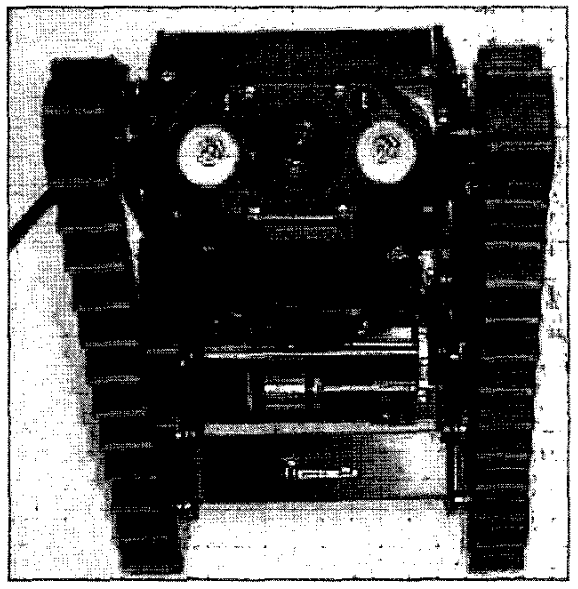
\includegraphics[width=0.5\textwidth]{robo-nao-antropomorfico.png} 
\caption{Robô utilizado em \citeonline{fin2004}}
\label{figure:caixa_sapato}
\end{figure}

Dois aspectos chamam a atenção em \cite{fin2004}. Ainda que a qualidade do rádio tenha sido o motivador para iniciar a comunicação via robô a comunicação não verbal foi mais abundante no fim do experimento. Isso ocorre porquê o ambiente de trabalho dessas equipes costuma ser bastante ruidoso, o que também nos indica que o robô deve ser capaz de reconhecer uma gama de gestos. O outro aspecto é a não necessidade de características antropomórficas para que haja uma comunicação homem máquina. Desde que haja algo que os demais membros do time possam reconhecer, ainda que de maneira bastante abstrata, como uma face é o suficiente para a comunicação.

De fato em \cite{akgun2022using} uma melhoria na iteração entre o time humano e o time de robôs é conseguido a partir de uma fita de leds que indica o humor do robô. A equipe que acompanha os robôs nos times de busca e salvamento muitas vezes não sabe se o robô está preso, e precisa de ajuda, ou apenas está performando alguma tarefa. É importante ressaltar que em um ambiente estressante essa dúvida se transforma em desconfiança o que pode reduzir a iteração homem máquina.

A liberdade do robô conseguir se expressar sem necessariamente ser antropomórfico é importante pois, como lembrado em \cite{habib2011} robôs de busca e salvamento são uma classe especial de robôs sociais por operarem em ambientes inóspitos. Dessa maneira o equipamento deve estar adaptado a sua missão: adentrar espaços confinados com dimensões muito estreitas, voo em áreas restritas, percorrer tubos, movimentação em terreno acidentado, capacidade de ascensão e descida verticais etc... E utilizar de alguns componentes para o aspecto de comunicação não verbal.

Em \cite{habib2011} é feita uma lista de requisitos para um robô de resgate e salvamento. Ainda que não exaustiva trata-se de uma lista bastante abrangente e abordá-la como um todo está além da proposta desse trabalho. Porém destacamos os seguintes pontos:

\begin{citacao}
O robô deverá detectar obstáculos, explorar seus arredores e navegar com segurança entre as estruturas colapsadas;

O robô deverá construir mapas e se localizar no mapa construído;

O robô deverá operar em vários módulos: remotamente operado, semi-autônomo, autônomo;

Humanos podem ser membros da equipe de robôs com diferentes funções;

O robô deverá captar sinais de áudio que sejam pistas da localização das vítimas e interpretá-los de maneira correta;

O robô deverá se comunicar com humanos e outros robôs de maneira confiável e inequívoca \cite{habib2011}.
\end{citacao}

Em \cite{tardioli2016} é exibida uma aplicação mais moderna de robôs de resgate e salvamento. A tecnologia de LIDAR permite a criação de um mapa, removendo assim uma das tarefas do operador responsável por criar a consciência situacional do robô em \cite{Robin2004}. São definidos apenas objetivos de alto nível e a partir do reconhecimento do terreno o robô é capaz de planejar seu avanço no espaço confinado. Outra questão também é tratada em \cite{tardioli2016} que é a necessidade de criação de uma rede de maneira automática para possibilitar a comunicação entre o robô e a base. Ainda que o robô possa ter alguma consciência situacional ele deve transmitir seus dados para o Posto de Comando a fim de que se tenha uma consciência global da situação.

Ainda que as 48 horas iniciais sejam as mais críticas para equipes de busca e salvamento, o atendimento a desmoronamentos e rompimento de barragens é uma tarefa que se alonga no tempo, podendo levar meses. Dessa maneira em \cite{krui2015} é avaliada a necessidade da construção de um relacionamento de tempo longo entre o time de robôs e o time humano. Para tal o robô deve ser capaz de reconhecer seus limites, solicitar ajuda de um operador humano e depois aprender com as atitudes tomadas pelo operador humano. Todas as informações coletadas pelos robôs também devem alimentar o Posto de Comando, dessa maneira, com o tempo, se terá um mapa cada vez mais detalhado da situação.

Por fim vários autores : \cite{Robin2004}, \cite{akgun2022using}, \cite{habib2011} chamam a atenção que o robô também deve ter a capacidade de se relacionar com as vítimas. Pois, aos olhos dessa o robô é um ponto de presença da equipe de salvamento, uma promessa de salvamento. Em \cite{Robin2004} ainda é trazido o fato que muitas vezes as equipes de salvamento localizam vítimas, mas são obrigadas a abandoná-las por alguma ordem do oficial de segurança, o robô, no entanto, não precisa ser evacuado sendo uma companhia para a vítima que espera ser socorrida. Como apontado pelos autores as capacidades empáticas para executar essa tarefa são bem maiores que as para cooperar com o time de resgate e não serão abordadas nesse trabalho.

\section{Modelo}
O modelo de robô a ser desenvolvido deverá atender os requisitos apresentado anteriormente. Porém o último requisito, por ser muito abrangente, será melhor especificado da maneira que se seque:

\begin{itemize}
\item O robô deverá reconhecer gestos simples como: siga, pare, esquerda, direita;
\item O robô deverá possuir um meio de comunicação não verbal que seja visível no ambiente da Zona Quente;
\item O robô deverá reconhecer comandos de voz simples: siga, pare, esquerda, direita;
\item Ainda que seja pouco utilizado na Zona Quente o robô deverá possuir caixas de som, a fim de ser uma presença avançada do Posto de Comando.
\end{itemize}

Para o processo de modelagem utilizar-se-á o arcabouço disposto em \cite{baraka2020}

\postextual

% ----------------------------------------------------------
% Referências bibliográficas
% ----------------------------------------------------------
\bibliography{abntex2-modelo-references}

% ----------------------------------------------------------
% Agradecimentos
% ----------------------------------------------------------

\section*{Agradecimentos}
Texto sucinto aprovado pelo periódico em que será publicado. Último 
elemento pós-textual.

\end{document}
